\documentclass{acm_proc_article-sp}
\usepackage[english]{babel}
\usepackage{graphicx}
\usepackage{url}
\usepackage{booktabs}

\setlength{\heavyrulewidth}{1.2pt}
\setlength{\lightrulewidth}{0.7pt}

\begin{document}

% na zaciatku som zadefinoval nadpis dokumentu a autorov

\title{Reducing the Sparsity of Contextual Information for Recommender Systems}

\numberofauthors{2}

\author{
\alignauthor
Dusan Zelenik\\
       \affaddr{Faculty of Informatics and Information}\\
       \affaddr{Technologies}\\
       \affaddr{Slovak University of Technology}\\
       \affaddr{Bratislava, Slovakia}\\
       \email{zelenik@fiit.stuba.sk}
\alignauthor
Maria Bielikova\\
       \affaddr{Faculty of Informatics and Information}\\
       \affaddr{Technologies}\\
       \affaddr{Slovak University of Technology}\\
       \affaddr{Bratislava, Slovakia}\\
       \email{bielik@fiit.stuba.sk}
}

\maketitle

% nasledne som si rozdelil cely dokument na kapitoly a podkapitoly, pouzil som prikazy section a subsection

\begin{abstract}
Our work focuses on the improvement of the accuracy of
context-aware recommender systems. Contextual informa-
tion showed to be promising factor in recommender systems.
However, pure context-based recommender systems can not
outperform other approaches mainly due to high sparsity
of contextual information. We propose an idea to improve
accuracy of context based recommender systems by context
inference. Context inference is based on effect discovered
by analyses of the context as a factor in
uencing user needs.
Analyses of the news readers reveals existence of behavioural
correlation which is the main pillar of proposed context infer-
ence. Method for context inference is based on collaborative
filtering and clustering of web usage (as a non-discretizing
alternative to association rules mining).
\end{abstract}

\category{H.3}{Information Storage and Retrieval}{Clustering In-
formation Filtering}
\category{H.2}{Database Applications}{Data
mining}

\terms{Algorithms}

\keywords{context, recommender system, clustering, user behaviour}


\section{MOTIVATION}
Context-aware recommender systems have become very
popular since variety of contextual information could be ac-
quired. With an increase of the smart-phone popularity and
available features which they provide, we are able to asso-
ciate user needs with contextual information. From the high
level context types such as location, time, weather, to the
low level context types such as humidity, noise, movement,
we study the impact of the context on the user behaviour and
needs. However context itself has shown to be insuficient
when it comes to accuracy of context-aware recommender
systems. Context is therefore used as a secondary aspect for
generating recommendation.

One reason for low accuracy is high sparsity of contex-
tual information. High sparsity is caused by various natures
of users and their preferences ~\cite{carlson2011wide}. Some users do not want
to share their personal information such as location, thus
causing missing contextual information. Poor context infor-
mation leads to low accuracy in prediction. On the other
hand, some users are willing to expose even personal con-
textual information such as emotions. They are willing to
answer question and explicitly express contextual informa-
tion, which is then useful in context-aware recommendation.

Our idea is to propagate contextual information from one
user to another in order to reduce the sparsity of data. We
propose the propagation of the context by exploiting a corre-
lation in users' behaviour. We assume that users' behaviour
is not random, it is based on context of the user. For in-
stance, Perse discovered association between negative
mood and tendency to watch competition-style programs as
a result of the need to experience happiness. Action-style
programs are selected when viewers are in a positive emo-
tional state. However, even if some associations are valid
for majority of users, we expect that there are associations
which could be discovered only for a subset of users. This
leads to clustering of users by their behaviour. Identifying
clusters of similar users helps to identify how to propagate
the context between users.

We discover associations between the need and context
using alternative to standard association rules mining. The
difference is in non-discrete values which we use. For exam-
ple, wrong discretization causes noise, as we lose the ability
to compare them and thus sort them. Therefore we expect to
achieve higher accuracy when we use proposed value based
associations discovery instead of item based. To accom-
plish value based associations discovery we combine stan-
dard techniques from machine learning such as x-means ~\cite{pelleg2000x}
and vector distance computation (Euclidean distance).

\section{RELATED WORK}
Context inference has received relatively little attention
in the literature when it comes to implicit inference from the
logs of user activity. It is caused by the selective approaches
to context incorporation. Specific solutions work with specific contextual information. Kahng et al. demonstrate
the predefined context as one of the factors for document
ranking in information retrieval process. As an example
they introduce weather and its impact on the user's inter-
est in song listening. This empiric context selection emerges
from the observation made by Baltranus et al. ~\cite{baltrunas2011context}. They research the relevance of the context in the system explicitly
by asking the user. They showed that supposed context has
positive impact on the success of their method. On the other
hand, research by Asoh et al. ~\cite{asoh2010analysis} proves that there is a signif-
icant difference between the real and supposed reaction to
the context. One way or another, this could be understood
as an explicit form of the context acquisition. And unfortu
nately, we are still unable to persuade and engage everyone
into explicit feedback.

Therefore we work with the acquired context and users'
behaviour to infer missing contextual information. To stress
the unavailability of contextual information we pick the work
of Bermingham et al. ~\cite{bermingham2010classifying}. They propose a solution to discover
the sentiment from microblogs. The sentiment is a deriva-
tion of the emotional context. Microblogs are perfect source
for discovering this type of the context. However it is do-
main specfic and could not be used as a generic solution.

Riboni et al. announced a hybrid of statistical analyses and ontological reasoning in order to acquire the context. Utilization in the COSAR project shows better results
by combining both of these approaches. We have decided
to use statistical approach boosted by empirically observed
effect of users behaviour correlation. We understand the
correlation of the behaviour as the correlation of the con-
textual information. Konomi et al. present connections
between people formed by co-presence at places. These con-
nections are based on geo-location but correlate with social
connections.

User behaviour is often represented by a set of actions performed by the user. Kramar observed the effect of changing the behaviour with the change of current context. He identified that multiple personas are present in the be-
haviour of individual. The same effect was exploited by
Park et al. . They clustered user's behaviour by actions
to improve query suggestions. They have actually used client
side logs to cluster the behaviour, which outperformed the
state-of-art approaches. From multiple personas of an indi-
vidual, we expanded to multiple personas of all users in the
system. Our intention is to supplement missing contextual
information using multiple personas.

Combining multiple personas of more users will improve
results in context inference. Research made by Cadiz et al. ~\cite{cadiz2009orchestrating}
or Rahnama et al. enables us to work with more users
and in various systems. By using standardized frameworks
and unifying context-aware systems, we are able to gather
usage logs. Contextual information on activities from vari-
ous systems improves our abilities to infer missing context.
The only drawback of such framework is the redundancy of
some information and higher complexity. Including informa-
tion on the past, present and future context increases
the complexity even more. Several approaches have been
presented to address this problem. Komninos et al. work
with vector representation of action and propose solution
to reduce complexity, even the complexity caused by vector
weighting issues. Reduction of the complexity is important
even for mobile devices where computational resources are
constrained. Dargie et al. discuss the need to reduce time
to recognise the context and its essence in real-time systems.

\section{CORRELATION IN SIMILAR USERS' BEHAVIOUR}
We have studied the effect of correlation in users' be-
haviour to propose an exploitation which would help to re-
duce the sparsity of contextual information. Our idea is to
propagate contextual information only to users whose be-
haviour highly correlates.

% v nasledujucom odstavci som vytvoril odkazy na poznamky pod ciarov

\subsection{Contextual Information}
To prove our concept we have decided to work with database
of web usage recorded by news portal SME.sk\footnote{http://www.sme.sk}. This news
portal is the biggest local news portal with more than 20
thousands active readers at the peak. Every click recorded
includes time, IP address, user identifier and article identifier. Further information such as category, section, author, publishing time for article are also provided. We used
this database before for content-based recommendation
which enables us to compare results achieved by our previ-
ous work.
To prepare database for further research, we add the con-
text which is not in database. We use services such as
wunderground\footnote{http://www.wunderground.com} and ip2location\footnote{http://www.ip2location.com} to add information on
weather and location. We also process timestamp to store
time derivatives (such as day of week, part of day, etc.).
Location which is extracted from IP address is very rough
and for dynamic block of IP addresses, the location is al-
most untraceable. We have also applied a simple rule based
algorithm to extract information on location (home, work,
outside) using time and IP address. It is based on repeat-
ing IP addresses during work days (from 8 AM to 5 PM),
during night and weekends. If the IP address was used by
user during work hours many times, we add the context of
location respectively (at work).
Dataset prepared in this way contains contextual informa-
tion which is acquired with both high and low confidence.
Low confidence causes sparsity what negatively affects fur-
ther recommendation process.

\subsection{User habits}
We have analysed news reading with focus on various con-
text types. We presume that user has habits which are af-
fected by context. We also presume that some users have
similar habits thus their behaviour is affected by context
similarly. We have mostly analysed the time as the most
popular context (see Fig. \ref{graf}). The figure shows that ma-
jority of users are in
uenced by forthcoming events. The
figure proves that majority of users have similar habits. For
instance, they read about cooking, when they are going to
cook for Christmas.
We also recognized same habits in smaller groups of users.
For example, local football games are commented on this
site, which attracts some users with interest in football.
These users have same interests. It could also mean that
these people are also similarly in
uenced by the same con-
text. In
uence of context means correlation in their be-
haviour. We use this effect of correlation in behaviour to
form clusters of similar users. Knowing similar users enables
us to propagate contextual information correctly.

% do dokumentu som vlozil obrazok a pridal som mu popis

\begin{center}

\textbf{Percentual share of displayed articles during a year
(shares for three different categories)}

\end{center}

\begin{figure} [ht]
\centering
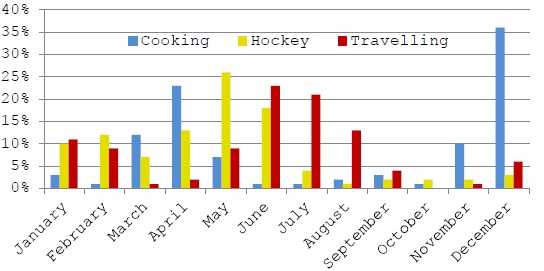
\includegraphics[width=0.4\textwidth]{images/graf.png}
\caption{Readers are influenced by forthcoming
events. We can observe the impact as an increase of
displayed articles on specific topics (monitoring real
users at SME.sk).}
\label{graf}
\end{figure}

\section{USER MODEL ENRICHMENT}
Our user model represent the measure of user interest in
item. Similarly to association rules we work with patterns.
Every pattern consist of a condition and filter. In our case
of news recommending, the filter is a combination of the
section and the category in news portal. There are around
420 combinations which could be used.
Condition expresses the context of the user which has to
be valid when the rule is applied to recommendation process.
We understand condition as a set of contexts which form a
condition together. Conditions are used to find situation of
the user. Condition and current situation of the user must
be matching when we want to apply the filter.
User model contains only the most frequent patterns. But
even if condition does not match current situation of the
user, we are still able to find the best matching condition.
Every context has its value which represents the importance
with a condition. Calculation of vector distances between
conditions and situation of the user results in best matching
rule which is then applied.

\subsection{Context Inference}
We have build the user model by processing user activity
which has been already recorded. Some contextual informa-
tion could be acquired directly using services and processing
attributes. However, some contextual information could be
missing or the confidence of the information is very low. We
propose the context inference which leads to the reduction
of the sparsity. Table (see Tab. \ref{tabulka}) demonstrates how could
the contextual information be propagated to another. These
actions could be represented as vectors and clustered using
all attributes except missing location. User A has complete
contextual information in this example. User B is considered
to be similar to User A since their behaviour is similar. In
result, contextual information for missing values is inferred
using known values and similar actions.

% vytvoril som numericky zoznam a pridal som do neho matematicky vzorec

\begin{enumerate}
		\item \textbf{Cluster users' actions.} User identifier is ignored at
this moment. We use x-means clustering ~\cite{pelleg2000x}.
		\item \textbf{Compute users' similarity.} Co-presence of actions
made by different users reveals their behavioural similarity.

		$$ similarity(u,v) = \frac {\sum_{i=0}^{n} ( \left|U  \cap C_i\right|  + \left|V  \cap C_i\right| )} {\left|U\right| +  \left|V\right|}$$

where U and V are sets of actions for users u and v
and C is the set of clusters.
		\item \textbf{Find the best matching actions.} Only actions of
similar users are used.
		\item \textbf{Propagate contextual information.} Only in case
it is available.
\end{enumerate}

% vytvoril som tabulku s udajmi a pridal som jej popis

\begin{table}[t]
\centering
\caption{Example of context inference. Actions 1, 2
are similar to actions 6, 7. Unknown context of lo-
cation could be propagated to user B using known
location from user A.}
\label{tabulka}
\begin{tabular}{@{}|c|c|c|c|c|c|@{}}
\toprule
action & user & \begin{tabular}[c]{@{}c@{}}hour\\ in day\end{tabular} & \begin{tabular}[c]{@{}c@{}}day in\\ week\end{tabular} & section & location \\ \midrule
1      & A    & 22                                                    & 2                                                     & sport   & work     \\
2      & A    & 21                                                    & 3                                                     & sport   & work     \\
3      & A    & 11                                                    & 7                                                     & cooking & home     \\
4      & A    & 11                                                    & 7                                                     & cooking & home     \\
5      & A    & 12                                                    & 7                                                     & cooking & home     \\
6      & B    & 19                                                    & 3                                                     & sport   & N/A      \\
7      & B    & 18                                                    & 5                                                     & sport   & N/A      \\
8      & B    & 12                                                    & 7                                                     & cooking & N/A      \\
9      & B    & 12                                                    & 7                                                     & cooking & N/A      \\
10     & B    & 13                                                    & 7                                                     & cooking & N/A     
\end{tabular}
\end{table}



Context inference is followed by enriching the user model.
It is done by finding the most frequent actions and extraction
of conditions and associated items. In order to keep values
not discretized we use clustering to find clusters of similar
actions per user. Complexity of such computation is however
very high, thus we process only the most recent actions. This
also keeps the user model up-to-date.

\subsection{Recommendation}
There are more options how to incorporate context into
recommender systems. Our user model enables us to rec-
ommend items by filtering them using rules stored in the
model. Current situation of the user is used to find the best
matching items. Items are used as filters on the dataset of
potential recommendations. Here we can work with content-
based approaches, collaborative filtering or other.
Content-based recommendation is generated using items
which are fetched from the model using current user con-
ditions. In this alternative we are searching for the items
in the dataset which are similar to items from user model.
Item in the user model is not necessarily one of items in
dataset. It could be only the set of keywords. We propose
to use category and section in our dataset of news.
Collaborative filtering is another very popular approach
to generate recommendations. To use our model with this
approaches we change the pair of condition and item to con-
dition and user. This enables us to reveal the most similar
users whose situations were very similar to the current situ-
ation of the user.

\section{EVALUATION STRATEGY}
As we already mentioned we work with database where
both low and high confident contextual information is present.
We propose to evaluate our method for sparsity reduction by
using only records with high confident contextual informa-
tion. We randomly select contextual information and sim-
ulate its confidence to be very low. Then we apply context
inference and compare inferred results with original values.
We also propose evaluation for context-aware recommen-
dation. We want to compare results achieved by recom-
mending news both with and without inferred contextual
information. Experiment is conducted with real people who
are separated into two groups. One group receives recom-
mendations generated only with original contextual infor-
mation. Another group receives recommendations generated
with inferred context (reduced contextual sparsity). In this
case we also incorporate test for statistical significance.
Another approach to evaluate our approach to sparsity
reduction is to compare our recommender system to others
to show expected improvement.

\section{CONCLUSIONS AND FUTURE WORK} 
In our work we face significant drawback of common spar-
sity in contextual information. We presented our proposal
for solving sparsity in contextual information using context
inference. We showed analyses of the web usage for news
portal and revealed the effect of behavioural correlation.
Clustering users by the web usage splits users with simi-
lar preferences into groups where the association between
context and need is also similar. In such group we can
propagate missing contextual information or context value
which is lacking in confidence. Our approach solves prob-
lems which are often present in frameworks which are gath-
ering contextual information from more sources.
In our future work we plan to generate news recommen-
dations using inferred context and compare results to our
previous work where we used pure content-based recommen-
dations. We also plan to apply this method for smart-
phones where we encounter higher variety of context types.
Context which could be acquired on smart-phone is more
complex than on the web what is big challenge for us.
Our main contribution is in reducing the sparsity of con-
textual information thus improving accuracy of context-aware
recommender systems. We have also designed an alternative
to association rules mining which respects numeric values.

\section{ACKNOWLEDGMENTS}
This work was partially supported by the Scientific Grant
Agency of the Ministry of Education of Slovak Republic,
grant VG1/0675/11 and by the Slovak Research and Devel-
opment Agency under the contract No. APVV-0208-10.

% nalinkoval som dokument, aby cital bibliografiu zo suboru "zdroje"

\bibliographystyle{abbrv}
\bibliography{zdroje}

\balancecolumns

\end{document}
